\section{Introduction}
%PUT IT ON ZENODO
The Sun's activity during the month of April 2022 was high. Indeed, 12 out of the 50 strongest Earth directed solar flares of the year were detected in that only month\footnote{\url{https://www.spaceweatherlive.com/en/solar-activity/top-50-solar-flares/year/2022.html}}. Moreover, 159 coronal mass ejections (CMEs) were detected by the LASCO instrument aboard SOHO in April 2022\footnote{\url{https://www.sidc.be/cactus/catalog.php}}. This is a $\sim$ 79\% increase compared to the 5 precedent months. Combined with an elongation of Venus near its maximal value, the observation conditions of this planet in the high-energy ranges were close to optimal. This report presents the approach used to recover the flux from a moving object, Venus, in the 3-10 keV energy range using the data from the JEM-X instrument aboard the \textit{INTEGRAL} telescope. The values detected from Venus' position is then compared to the Sun's activity during that period.

This \textbf{Introduction }section first presents the telescope and instrument used. Then the data retrieving method using the \textit{Online Data Analysis - Application Programming interface} of \textit{INTEGRAL} is described. The main channels X-Rays emission of planets is finally discussed.

The \textbf{Observation, data analysis and methods} section shows the steps in the selection of the data, the criteria, assumptions and models used
\subsection{INTEGRAL telescope}
    
    \begin{figure}[H]
        \centering
        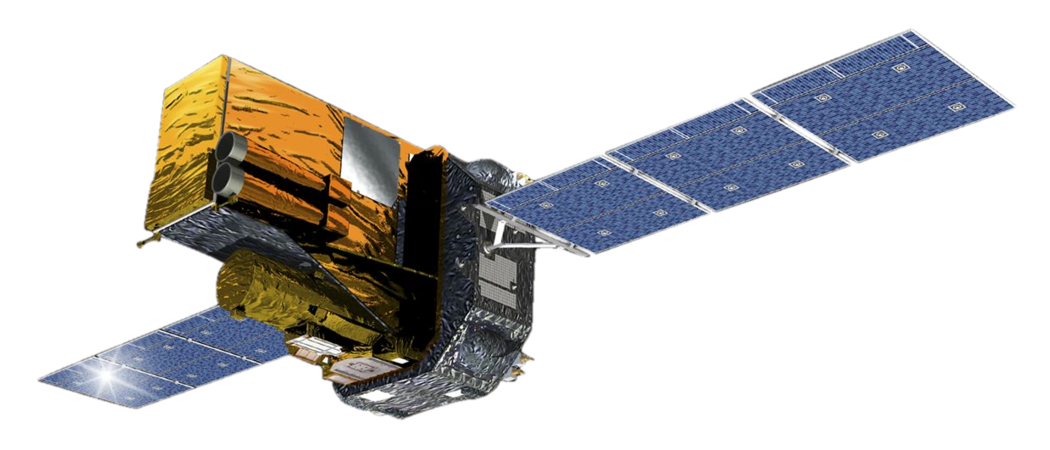
\includegraphics[width = 8cm]{report/Figures/intro/INTEGRAL_spacecraft_model.png}
        \caption{Caption}
        \label{integral}
    \end{figure}
    
        \subsection{JEM-X detector}
        
        \begin{figure}[H]
        \centering
        \begin{subfigure}{.45\textwidth}
            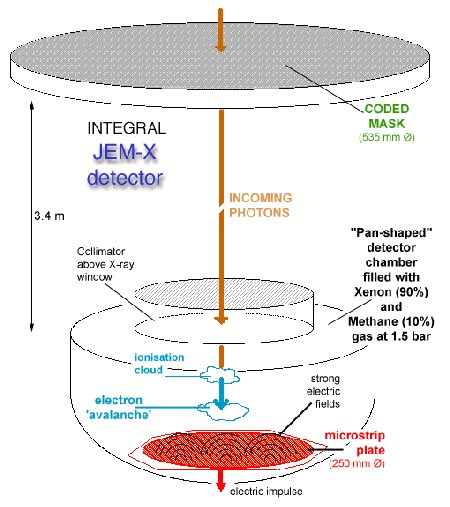
\includegraphics[width=\textwidth]{report/Figures/intro/jem_x_funct_diagram.jpg}
        \end{subfigure}%
        \hspace{1em}-
        \begin{subfigure}{.45\textwidth}
            \centering
            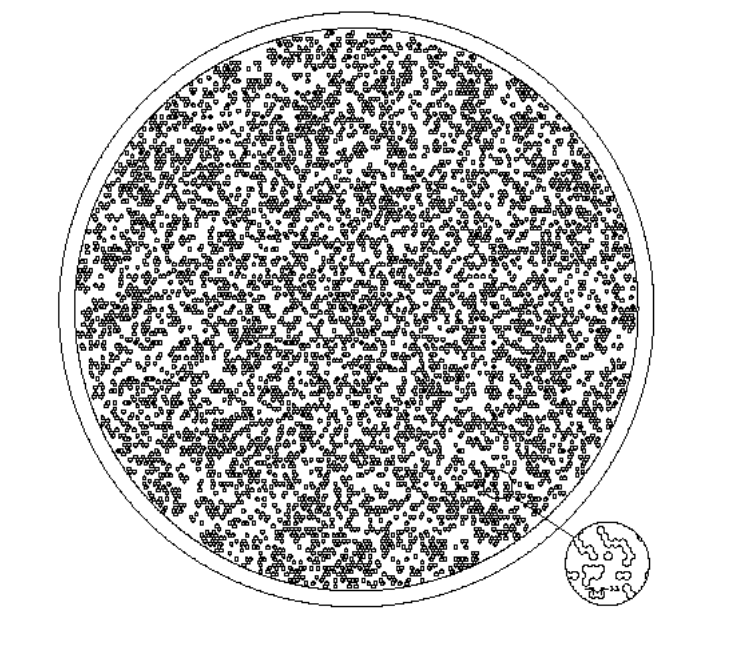
\includegraphics[width=\textwidth]{report/Figures/intro/jemx_coded_mask.png}
        \end{subfigure}
        \caption{}
        \label{jemx}
        \end{figure}
    

    \subsection{\texttt{ODA-API}}
    \subsection{X-Ray emission of planets}